\documentclass[tikz,border=6pt]{standalone}
\usepackage[T1]{fontenc}
\usetikzlibrary{positioning,arrows.meta,calc}
\begin{document}
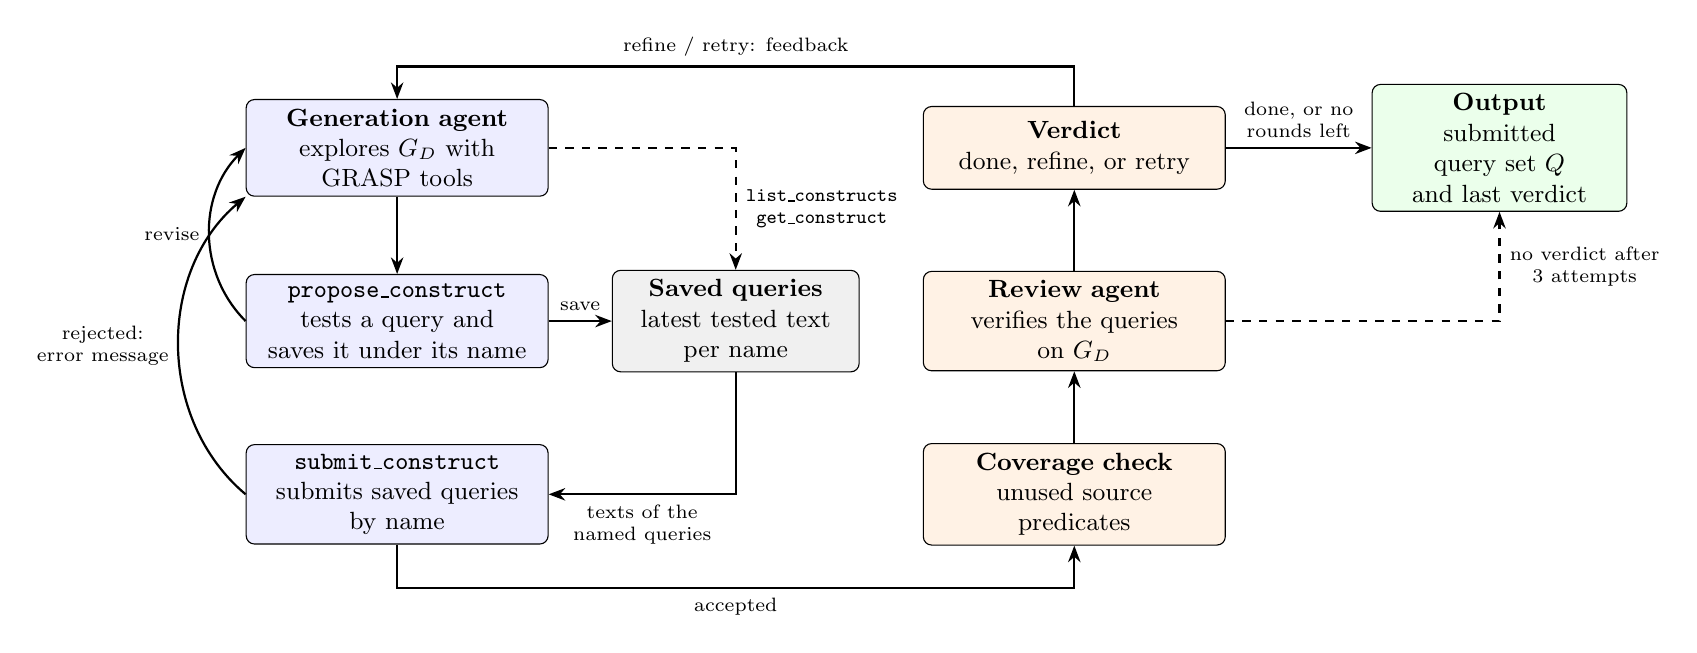
\begin{tikzpicture}[
  box/.style={draw, rounded corners=3pt, align=center, font=\small,
              minimum height=1.05cm, text width=3.6cm, fill=white},
  gen/.style={box, fill=blue!7},
  store/.style={box, fill=gray!12, text width=2.9cm},
  rev/.style={box, fill=orange!10},
  outbox/.style={box, fill=green!8, text width=3.0cm},
  arr/.style={-{Stealth[length=6pt]}, thick},
  lab/.style={font=\scriptsize, align=center}
]
% generation side
\node[gen]   (explore) at (0,0)     {\textbf{Generation agent}\\explores $G_D$ with\\GRASP tools};
\node[gen]   (test)    at (0,-2.2)  {\texttt{propose\_construct}\\tests a query and\\saves it under its name};
\node[gen]   (submit)  at (0,-4.4)  {\texttt{submit\_construct}\\submits saved queries\\by name};
\node[store] (saved)   at (4.3,-2.2) {\textbf{Saved queries}\\latest tested text\\per name};
% review side
\node[rev]   (cov)     at (8.6,-4.4) {\textbf{Coverage check}\\unused source\\predicates};
\node[rev]   (review)  at (8.6,-2.2) {\textbf{Review agent}\\verifies the queries\\on $G_D$};
\node[rev]   (verdict) at (8.6,0)    {\textbf{Verdict}\\done, refine, or retry};
% output
\node[outbox] (output) at (14.0,0)  {\textbf{Output}\\submitted query set $Q$\\and last verdict};

% generation loop
\draw[arr] (explore) -- (test);
\draw[arr] (test.west) to[bend left=45] node[lab, left]{revise} (explore.west);
\draw[arr] (test) -- node[lab, above]{save} (saved);
\draw[arr] (saved.south) |- node[lab, below, pos=0.75]{texts of the\\named queries} (submit.east);
\draw[arr, dashed] (explore.east) -| node[lab, right, pos=0.75]{\texttt{list\_constructs}\\\texttt{get\_construct}} (saved.north);
\draw[arr] (submit.west) to[bend left=50] node[lab, left, pos=0.5]{rejected:\\error message} (explore.south west);
% to review
\draw[arr] (submit.south) -- ++(0,-0.55) -| node[lab, below, pos=0.25]{accepted} (cov.south);
\draw[arr] (cov) -- (review);
\draw[arr] (review) -- (verdict);
% feedback
\draw[arr] (verdict.north) -- ++(0,0.5) -| node[lab, above, pos=0.25]{refine / retry: feedback} (explore.north);
% finish
\draw[arr] (verdict) -- node[lab, above]{done, or no\\rounds left} (output);
\draw[arr, dashed] (review.east) -| node[lab, right, pos=0.75]{no verdict after\\3 attempts} (output.south);
\end{tikzpicture}
\end{document}